\documentclass[12pt, a4paper]{article}
\usepackage{amsmath, amssymb, amsfonts} 
\usepackage{inputenc}
\usepackage{float}
\usepackage{graphics}                 
\usepackage{color}                    
\usepackage{hyperref}
\usepackage{ptext}
\usepackage{graphicx}                         
%\settextfont[Scale=.9]{Calibri}

%\graphicspath{ {images/} }

\hypersetup{
	colorlinks=true,
	linkcolor=blue,
	filecolor=magenta,      
	urlcolor=cyan
}


\title{
	{\Huge \textbf{In the name of God}}
	\\[20pt]
	
\includegraphics[width=0.5\linewidth]{../assets/IUST_logo_color_eng.jpg} \\
	{\normalsize Department of Computer Engineering}
}

\author{
	\\[10pt]
	\textbf{{\LARGE Natural Language Processing}}
	\\[10pt]
	\LARGE Final Phase Report
	\thanks{\url{https://github.com/yegmor/NLPProject}}
	
	\\[30pt]
	\textbf{Yeganeh Morshedzadeh}
	\\[5pt]
	Student Number: 96521488
}

\date{Spring 2021} 

\begin{document}
	
\maketitle
%\graphicspath{{../reports/images}}‎
	
\clearpage
%\addtocontents{toc}{\textbf{Content}~\hfill\textbf{Page}\par}
\tableofcontents
\newpage

\listoffigures
\newpage

\listoftables
\newpage

\begin{abstract}
	In this project, we tried to use Natural Language Processing to better understand Depression and Anxiety posts. The dataset is gathered from Reddit communities \href{https://www.reddit.com/r/depression}{r/depression} and \href{https://www.reddit.com/r/Anxiety}{r/Anxiety}.
	\\[10pt]
	
	For this project, at first, we wrote a project proposal (\href{https://docs.google.com/document/d/1tHGEmEgn8-sp8MD72d8NjnZsq-GpVupzsMWgnqaGi-Y/edit?usp=sharing}{Google Docs}), and afterwards, in the first phase (\href{https://docs.google.com/document/d/1Jc2ELhweU01Tbf0WalU7wVQABdAV4w50mhQnmMpU2mM/edit?usp=sharing}{Google Docs}), we gathered data and made some exploratory data analysis. 
	\\[10pt]
	
	In the final phase, we went deeper, and tried various NLP tasks, such as, computing Word2Vec, Tokenization, Parsing, and creating a language model based on our the dataset.
\end{abstract}

\newpage
\part{Word2Vec}
\large{\textbf{Filename:} 3\_word2vec.ipynb}

\section*{Code}
For this part we have three Word2Vec models, named as dep\_w2v\_model, anx\_w2v\_model, and all\_w2v\_model. Moreover, with boolean parameters, load and save, the model will be saved and/or loaded in the my\_word2vec function.

\begin{table}[ht]
	\caption{Word2Vec vocabulary size} 
	\centering 
	\vspace{5mm} 
	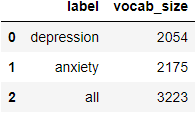
\includegraphics[width=0.5\linewidth]{../reports/images/w2v_vocab-size.png}
	\label{table:nonlin} 
\end{table}



\section*{Results and Examples}
To make the visualizations more relevant, we will look at the relationships between a query word (in \textcolor{red}{**red**}), its most similar words in the model (in \textcolor{blue}{**blue**}), and other words from the vocabulary (in \textcolor{green}{**green**})

\newpage
\part{Tokenization}
\large{\textbf{Filename:} 4\_tokenization.ipynb}

\section*{Code}
In this part we have used KFold to split our data into train and test. Afterwards, we train SentencePiece model based on the data. Lastly, we compute <UNK> on our test dataset. 

\section*{Results and Examples}


\newpage
\part{Parsing}
In this part, we used Stanza, which is a a Python NLP Package, and a collection of accurate and efficient tools for the linguistic analysis of many human languages. Starting from raw text to syntactic analysis and entity recognition, Stanza brings state-of-the-art NLP models to languages of your choosing.

More specifically, we used their \href{http://stanza.run/}{Online Demo} to create a manual .CoNLL file based on our dataset. Later, we can use \href{https://universaldependencies.org/conllu_viewer.html}{Universal Dependencies CoNLL viewer} to automatically generate parse tree from .CoNLL file.

\section*{Results and Examples}
\begin{enumerate}
	\item I never really showed any sadness when I am with someone.
	\item he is a good person, and I know that.
	\item how am I feeling?
	\item last year I went through a huge amount of stress.
	\item how can you tell the difference between an actual issue or anxiety?
	\item please do not judge.
	\item what do you think is the meaning of life?
	\item today was a very strange day.
	\item all these emotions are too much sometimes. 
	\item everybody is going to die.
\end{enumerate}

\newpage
\part{Language Model}
\large{\textbf{Filename:} 5\_language-model.ipynb}

\section*{Code}
In this part we have used KFold to split our data into train and test. Afterwards, we train SentencePiece model based on the data. Lastly, we compute <UNK> on our test dataset. 

\section*{Results and Examples}



\newpage
\part{Fine Tuning}

\section*{Classification}
\large{\textbf{Filename:} 6\_finetune\_classification.ipynb}

\subsection*{Code}
In this part we have used KFold to split our data into train and test. Afterwards, we train SentencePiece model based on the data. Lastly, we compute <UNK> on our test dataset. 

\subsection*{Results and Examples}
\section*{Language Model}
\large{\textbf{Filename:} 7\_finetune\_language-model.ipynb}

\subsection*{Code}
In this part we have used KFold to split our data into train and test. Afterwards, we train SentencePiece model based on the data. Lastly, we compute <UNK> on our test dataset. 

\subsection*{Results and Examples}

%
%\begin{figure}[H]
%	\centering{\includegraphics[width=\linewidth, height=\textheight, keepaspectratio]{images/table.png}}
%	\caption{جدول به ازای مقادیر مختلف n}
%	\label{table}
%\end{figure}


\newpage



\begin{thebibliography}{9}
	\bibitem{bib0}
	\url{https://towardsdatascience.com/goodbye-world-4cc844197d51}
	
	\bibitem{bib1}
	\url{https://colab.research.google.com/github/google/sentencepiece/blob/master/python/sentencepiece_python_module_example.ipynb#scrollTo=ee9W6wGnVteW}
	
	\bibitem{bib2}
	\url{https://gmihaila.github.io/tutorial_notebooks/gpt2_finetune_classification/}
	
	\bibitem{bib3}
	\url{https://colab.research.google.com/github/philschmid/fine-tune-GPT-2/blob/master/Fine_tune_a_non_English_GPT_2_Model_with_Huggingface.ipynb#scrollTo=hKBSyNLgqF9K}
	
	\bibitem{bib4}
	\url{https://github.com/huggingface/notebooks/blob/master/examples/language_modeling.ipynb}
	
	\bibitem{bib5}
	\url{https://www.kaggle.com/pierremegret/gensim-word2vec-tutorial}
	
	\bibitem{bib6}
	\url{https://machinelearningmastery.com/how-to-develop-a-word-level-neural-language-model-in-keras/}
	
	\bibitem{bib7}
	\url{https://huggingface.co/transformers/training.html}
	
	\bibitem{bib8}
	\url{https://www.kaggle.com/achintyatripathi/gensim-word2vec-usage-with-t-sne-plot}
	
	\bibitem{bib9}
	\url{https://colab.research.google.com/github/borisdayma/huggingtweets/blob/master/huggingtweets-demo.ipynb}
	
	\bibitem{bib10}
	\url{https://huggingface.co/transformers/custom_datasets.html}
	
	\bibitem{bib11}
	
\end{thebibliography}

\end{document}          
